\documentclass[tikz,border=10pt]{standalone}
\usepackage{amssymb} % for \subset
\usepackage{pgf,tikz,pgfplots,tkz-euclide}
\usepackage{tikz-3dplot}
\pgfplotsset{compat=1.15}
\usepackage{mathrsfs}
\usepackage{amsmath}
\allowdisplaybreaks[4]
\usetikzlibrary{arrows,arrows.meta,angles,quotes,automata,math}
\usetikzlibrary{calc,fadings,decorations.pathreplacing}
\usetikzlibrary{shadings,intersections}
\usetikzlibrary{3d}
\usetikzlibrary{hobby}
%\usepackage{amsthm}
\usepackage{wrapfig}
\usepackage{gensymb}
\usepackage{subfigure} 
\usepackage{physics}
\usepackage{diagbox}

\begin{document}

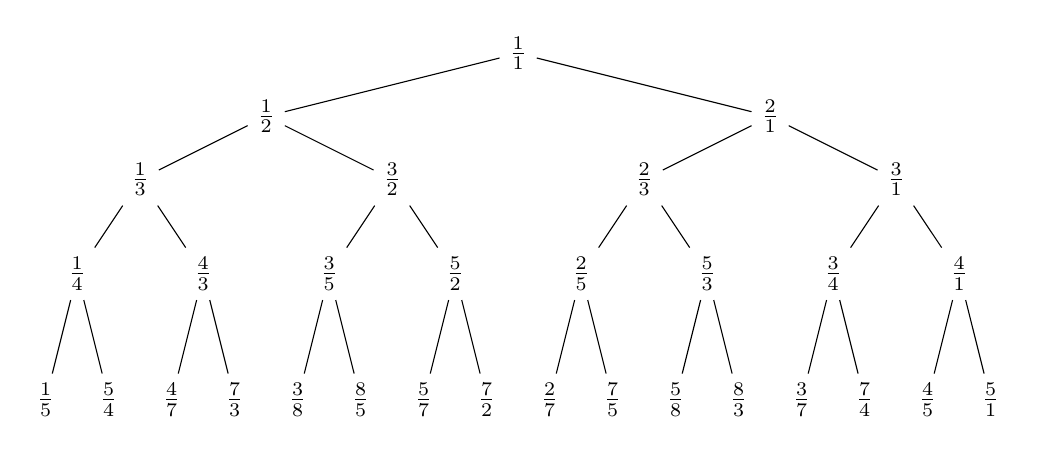
\begin{tikzpicture}[scale=0.8]
\path
(0,0)     node[] (1) {$\frac{1}{1}$}
+(-4,-1) node[] (2) {$\frac{1}{2}$}
+(4,-1)   node[] (3) {$\frac{2}{1}$}
(2)
+(-2,-1)  node[] (4) {$\frac{1}{3}$}
+(2,-1)   node[] (5) {$\frac{3}{2}$}
(3)
+(-2,-1)   node[] (6) {$\frac{2}{3}$}
+(2,-1)  node[] (7) {$\frac{3}{1}$}
(4)
+(-1,-1.5) node[] (8) {$\frac{1}{4}$}
+(1,-1.5)  node[] (9) {$\frac{4}{3}$}
(5)
+(-1,-1.5) node[] (10) {$\frac{3}{5}$}
+(1,-1.5)  node[] (11) {$\frac{5}{2}$}
(6)
+(-1,-1.5) node[] (12) {$\frac{2}{5}$}
+(1,-1.5)  node[] (13) {$\frac{5}{3}$}
(7)
+(-1,-1.5) node[] (14) {$\frac{3}{4}$}
+(1,-1.5)  node[] (15) {$\frac{4}{1}$}
(8)
+(-.5,-2) node[] (16) {$\frac{1}{5}$}
+(.5,-2)  node[] (17) {$\frac{5}{4}$}
(9)
+(-.5,-2) node[] (18) {$\frac{4}{7}$}
+(.5,-2)  node[] (19) {$\frac{7}{3}$}
(10)
+(-.5,-2) node[] (20) {$\frac{3}{8}$}
+(.5,-2)  node[] (21) {$\frac{8}{5}$}
(11)
+(-.5,-2) node[] (22) {$\frac{5}{7}$}
+(.5,-2)  node[] (23) {$\frac{7}{2}$}
(12)
+(-.5,-2) node[] (24) {$\frac{2}{7}$}
+(.5,-2)  node[] (25) {$\frac{7}{5}$}
(13)
+(-.5,-2) node[] (26) {$\frac{5}{8}$}
+(.5,-2)  node[] (27) {$\frac{8}{3}$}
(14)
+(-.5,-2) node[] (28) {$\frac{3}{7}$}
+(.5,-2)  node[] (29) {$\frac{7}{4}$}
(15)
+(-.5,-2) node[] (30) {$\frac{4}{5}$}
+(.5,-2)  node[] (31) {$\frac{5}{1}$}
;
\draw (2)--(1)--(3) (4)--(2)--(5) (6)--(3)--(7) (8)--(4)--(9) 
(10)--(5)--(11) (12)--(6)--(13) (14)--(7)--(15)
(16)--(8)--(17) (18)--(9)--(19) (20)--(10)--(21) (22)--(11)--(23)
(24)--(12)--(25) (26)--(13)--(27) (28)--(14)--(29) (30)--(15)--(31)
;
\end{tikzpicture}

\end{document}